\documentclass[10pt,a4paper]{article}
\usepackage[utf8]{inputenc}
\usepackage[french]{babel}
\usepackage[T1]{fontenc}
\usepackage{amsmath}
\usepackage{amsfonts}
\usepackage{amssymb}
\usepackage{graphicx}
\usepackage[left=2cm,right=2cm,top=2cm,bottom=2cm]{geometry}

\title{Équations de la fusée}
\author{Jonathan Plasse}

\begin{document}
	\section*{Équations de la fusée}
	\[\dfrac{\mathrm{d}p}{\mathrm{d}t}=\vec{P}+\vec{R}+m\vec{g}\]
	\[\|\vec{P}\|=146.7\ N\]
	\[\|\vec{g}\|=9.81\ m.s^{-2}\]
	\[\|\vec{R}\|=\frac{1}{2}\rho_0.e^{-z/h}S.C_x.\|\vec{v}\|^2\]
	\[m=m_{poidstotal}-\frac{t}{t_{combustion}}m_{carburant}\]
	\[\varphi=\arccos\frac{v_x}{\|\vec{v}\|}\]
	$\vec{P}$, $\vec{R}$ et $\vec{v}$ sont colinéaire à l'axe principal de la fusée

	Ainsi, on obtient ddz, ddx, dz, dx, x, z qui sont respectivement des accélérations, vitesses, positions.
	
	
	\[ddz = \frac{P-sign(dz)R_{air}(z, v)}{m(t)}\sin(\varphi)+D.dz-g\]
	\[ddx = \frac{P-sign(dz)R_{air}(z, v)}{m(t)}\cos(\varphi)+D.dx\]
	\[v=\sqrt{dz^2+dx^2}\]
	\[\varphi=\arccos\frac{dx}{v}\]
	\[\varphi_{initial}=80\frac{\pi}{180}\ rad\]
	\[m(t):t<t_{combustion}=m_{poidstotal}-\frac{t}{t_{combustion}}m_{carburant}\]
	\[m(t):t\ge t_{combustion}=m_{poidstotal}-m_{carburant}\]
	\[R_{air}(z,v)=\frac{1}{2}\rho_0.e^{-z/h}S.C_x.v^2\]
	\[D=\frac{m_{carburant}}{t_{combustion}}\]
	\[P=146.7\ N\]
	\[m_{poidstotal} = 1.6\ kg\]
	\[m_{carburant} = 0.0843\ kg\]
	\[t_{combustion} = 0.97\ s\]
	\[S = rayon^2\pi\]
	\[rayon = 0.04\ m\]
	\[C_x = 0.35\]
	\[hs = \frac{RT}{Mg}\]
	\[M = 0.028966\ kg.mol^{-1}\]
	\[g = 9.81\ m.s^{-2}\]
	\[R = 8.315\ J.mol^{-1}.K^{-1}\]
	\[T = 30+273.15\ K\]
	
	\begin{figure}[h]
		\centering
		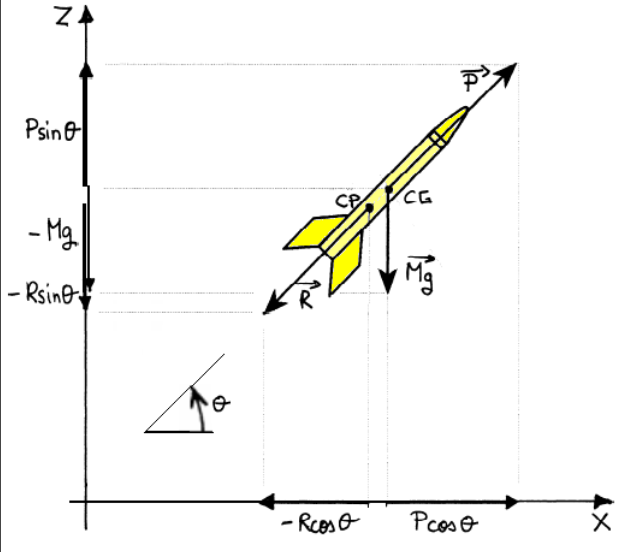
\includegraphics[scale=0.5]{fusee.png}
		\caption{Schéma des forces}
	\end{figure}
\end{document}